%----------------------------------------------------------------------------------------
%       PACKAGES AND OTHER DOCUMENT CONFIGURATIONS
%----------------------------------------------------------------------------------------
\documentclass[paper=a4, fontsize=12pt]{article}
\usepackage[german]{babel} % English language/hyphenation
\usepackage{amsmath,amsfonts,amsthm,mathtools} % Math packages
\usepackage[utf8]{inputenc}
\usepackage{float}
\usepackage{lipsum} % Package to generate dummy text throughout this template
\usepackage{blindtext}
\usepackage{graphicx} 
\usepackage[font={small,it}]{caption}
\usepackage{wrapfig} % Wrapping text around objects
\usepackage{subcaption}
\usepackage[sc]{mathpazo} % Use the Palatino font
\usepackage[T1]{fontenc} % Use 8-bit encoding that has 256 glyphs
\linespread{1.05} % Line spacing - Palatino needs more space between lines
\usepackage{microtype} % Slightly tweak font spacing for aesthetics
\usepackage[hmarginratio=1:1,top=32mm,columnsep=20pt]{geometry} % Document margins
%\usepackage[hang, small,labelfont=bf,up,textfont=it,up]{caption} % Custom captions under/above floats in tables or figures
\usepackage[hidelinks]{hyperref} % For hyperlinks in the PDF
\usepackage{lettrine} % The lettrine is the first enlarged letter at the beginning of the text
\usepackage{paralist} % Used for the compactitem environment which makes bullet points with less space between them
\usepackage{abstract} % Allows abstract customization
\renewcommand{\abstractnamefont}{\normalfont\bfseries} % Set the "Abstract" text to bold
\renewcommand{\abstracttextfont}{\normalfont\small\itshape} % Set the abstract itself to small italic text
\usepackage{titlesec} % Allows customization of titles
\setlength{\parindent}{0pt}

\renewcommand\thesection{\Roman{section}} % Roman numerals for the sections
\renewcommand\thesubsection{\Roman{subsection}} % Roman numerals for subsections

\titleformat{\section}[block]{\large\scshape\centering}{\thesection.}{1em}{} % Change the look of the section titles
\titleformat{\subsection}[block]{\large}{\thesubsection.}{1em}{} % Change the look of the section titles
\newcommand{\horrule}[1]{\rule{\linewidth}{#1}} % Create horizontal rule command with 1 argument of height
\usepackage{fancyhdr} % Headers and footers
\pagestyle{fancy} % All pages have headers and footers
\fancyhead{} % Blank out the default header
\fancyfoot{} % Blank out the default footer

\fancyhead[C]{Hamburg University of Applied Sciences $\,\bullet\,$ BTI3-ADP/01} % Custom header text

\fancyfoot[RO,LE]{\thepage} % Custom footer text

%----------------------------------------------------------------------------------------
%       SYNTAX HIGHLIGHTING
%
% Show available Languages: pygmentize -L
%----------------------------------------------------------------------------------------
\usepackage{minted}

\newminted{java}{autogobble, tabsize = 2, frame=single, breaklines, fontfamily=courier, fontsize=\footnotesize}
\newmintinline{java}{autogobble, fontfamily=courier, style=bw}

\newminted{c}{autogobble, tabsize = 2, frame=single, breaklines, fontfamily=courier, fontsize=\footnotesize}
\newmintinline{c}{autogobble, fontfamily=courier, style=bw}

\newminted{cpp}{autogobble, tabsize = 2, frame=single, breaklines, fontfamily=courier, fontsize=\footnotesize}
\newmintinline{cpp}{autogobble, fontfamily=courier, style=bw}

\newminted{php}{autogobble, tabsize = 2, frame=single, breaklines, fontfamily=courier, fontsize=\footnotesize}
\newmintinline{php}{autogobble, fontfamily=courier, style=bw}

\newminted{text}{tabsize = 2, frame=single, breaklines, fontfamily=courier, fontsize=\footnotesize}
\newmintinline{text}{fontfamily=courier, style=bw}

\newminted{bash}{autogobble, tabsize = 2, frame=single, breaklines, fontfamily=courier, fontsize=\footnotesize}
\newmintinline{bash}{autogobble, fontfamily=courier, style=bw}

\newminted{matlab}{autogobble, tabsize = 2, frame=single, breaklines, fontfamily=courier, fontsize=\footnotesize}
\newmintinline{matlab}{autogobble, fontfamily=courier, style=bw}

%----------------------------------------------------------------------------------------
%       TITLE SECTION
%----------------------------------------------------------------------------------------
\title{\vspace{-15mm}\fontsize{24pt}{10pt}\selectfont\textbf{Binärer Suchbaum Teil 2}} % Article title
\author{
\large
{\textsc{Aufgabenblatt 8}}\\[2mm]
{\textsc{Niels Gandraß (2285656)}}\\[2mm]
%{\textsc{Helena Lavjevardi (2250233)}}\\[2mm]
%{\textsc{Marcel Röthke (2298730)}}\\[2mm]
%{\textsc{Max Musterstudent (13374242) }}\\[2mm]
%\thanks{A thank you or further information}\\ % Your name
%\normalsize \href{mailto:marco.torres.810@gmail.com}{marco.torres.810@gmail.com}\\[2mm] % Your email address
}
\date{25. Mai 2017} % Uncomment to remove date

%----------------------------------------------------------------------------------------
\begin{document}
\maketitle % Insert title
\thispagestyle{fancy} % All pages have headers and footers


\begin{center}
	\textbf{Abstract}\\
	\textit{Es wird gezeigt wie die Summe der Elemente eines binären Suchbaums auf einem gegebenen Intervall möglichst effizient berechnet werden kann. Hierzu wird die Zusatzinformation "Summe der kleineren Knoten" in jedem Knoten des Baum hinterlegt. So kann durch finden der beiden Elemente, welche durch das gegebene Intervall eingeschlossen werden, direkt die Summe aller Knoten innerhalb des Intervalls bestimmt werden.}
\end{center}


\section{Vorwort}
Im Rahmen des achten Aufgabenblatts des Moduls BTI3-ADP wurde ein Verfahren entwickelt, welches es ermöglicht in binären Suchbäumen schnellstmöglich die Summe der Elemente, innerhalb eines gegebenen Intervalls, zu berechnen.

\begin{center}
	Enthält ein binärer Suchbaum die Elemente $F = a_1, a_2, \ldots, a_{n-1}, a_{n}$, so erfolgt die Berechnung der Summe durch:
\end{center}
$$ \sum_{i}^{} a_i ~~\text{mit}~~ m \leq a_i \leq M $$
\begin{center}
	Wobei $m$ der unteren und $M$ der oberen Intervall-Grenze entspricht.
\end{center}

\vspace{6pt}
Zur Umsetzung wurde in dieser Ausarbeitung die Programmiersprache Java\footnote{https://en.wikipedia.org/wiki/Java\_(programming\_language)} genutzt. Die, in ihrer Art, durchgeführten Untersuchungen können jedoch unabhängig der Programmiersprache nachvollzogen werden.

\section{Kurz und Knackig}
Durch das verwendete Verfahren lies sich die Berechnung der Summe auf die Komplexität für das Finden von Knoten im binären Suchbaum reduzieren. Somit wurde $\mathcal{O}(log(n))$ erreicht.

\newpage
\section{Implementiertes Verfahren}
Es wurde ein Verfahren implementiert, welches in jedem Knoten des binären Suchbaums eine Zusatzinformation hinterlegt. Es wird die Summe der kleineren Knoten gespeichert. Somit kann durch finden der beiden Elemente, welche durch das gegebene Intervall eingeschlossen werden, direkt die Summe aller Knoten innerhalb des Intervalls bestimmt werden.

\subsection{Berechnen der Zusatzinformation}
Diese Summe wird mit Aufruf von \javainline{updateChildSums()} aktualisiert. Hierbei wird der Baum in Inorder-Reihenfolge traversiert und jeweils die Werte der Knoten aufaddiert und in den nächsten Knoten geschrieben.

\begin{javacode}
/**
 * Wrapper for updateChildSums(LinkedBinaryTreeNode, Long)
 */
public void updateChildSums() {
	updateChildSums(_rootNode, 0L);
}

/**
 * Iterates inOrder trough the tree and sums up all values that are smalle than curNode
 *
 * @param curNode Current node to process
 * @param curSum  Current sum
 *
 * @return Current sum after calculation to destruct call stack
 */
private Long updateChildSums(LinkedBinaryTreeNode curNode, Long curSum) {
	// Cancelation condition
	if (curNode == null) {
		return 0L;
	}
	
	// Go down do smallest (leftest) node
	if (curNode.getLeftChild() != null) {
		curSum = updateChildSums(curNode.getLeftChild(), curSum);
	}
	
	// Add curNodes value to sum
	curSum += curNode.getValue();
	curNode.setLowerValueSum(curSum);
	_counterUpdateChildSum++;
	
	// Go down to biggest (rightest) node
	if (curNode.getRightChild() != null) {
		curSum = updateChildSums(curNode.getRightChild(), curSum);
	}
	
	return curSum;
}
\end{javacode}

\newpage
\subsection{Berechnen der Knotensumme}
Zur Berechnung der Summe der Knoten des binären Suchbaums auf deinem gegebenen Intervall müssen nun nur noch die umschließenden Knoten gefunden werden. Somit wird für den Knoten, welcher die obere Grenze bildet der nächst größere Knoten gesucht. Für den Knoten, welcher die untere Grenze bildet, der nächst kleinere.\\
\\
Abschließend werden von Unterknotensumme des oberen Kontens die Unterknotensumme des unteren Knotens und gegebenenfalls ein Offset abgezogen. Dieser Offset berücksichtigt den Sonderfall, dass beispielsweise die Grenze genau auf einem vorhandenen Knoten liegt.

\begin{javacode}
/**
 * Determines the sum of node values between the given bounds
 *
 * @param lowerBound Lower bound
 * @param upperBound Upper bound
 *
 * @return Sum of the node values in between these bounds
 */
public Long limitSum(long lowerBound, long upperBound) {
	// Preconditions
	if (lowerBound > upperBound)
	throw new IllegalArgumentException();
	
	// Find nodes
	LinkedBinaryTreeNode upperNode = findClosestBiggerNode(upperBound);
	LinkedBinaryTreeNode lowerNode = findClosestSmallerNode(lowerBound);
	
	// Assure that nodes got found otherwise select smallest/biggest node
	if (upperNode == MIN_VALUE_NODE) {
		upperNode = getBiggestNode();
		upperBound = upperNode.getValue();
		_counterLimitSum++;
	}
	if (lowerNode == MAX_VALUE_NODE) {
		lowerNode = getSmallestNode();
		lowerBound = lowerNode.getValue();
		_counterLimitSum++;
	}
	
	// Calculate offset for cases where nodes match directly
	long offset = 0;
	if (lowerNode.getValue() == lowerBound)
	offset += lowerNode.getValue();
	if (upperNode.getValue() > upperBound)
	offset -= upperNode.getValue();
	_counterLimitSum+=2;
	
	// Calculate difference
	_counterLimitSum++;
	return findClosestBiggerNode(upperBound).getLowerValueSum() - findClosestSmallerNode(lowerBound).getLowerValueSum() + offset;
}
\end{javacode}

\newpage
\subsection{UML-Klassendiagram}
Folgendes UML-Klassendiagram zeigt die komplette Implementierung.

\begin{figure}[H]
	\centering
	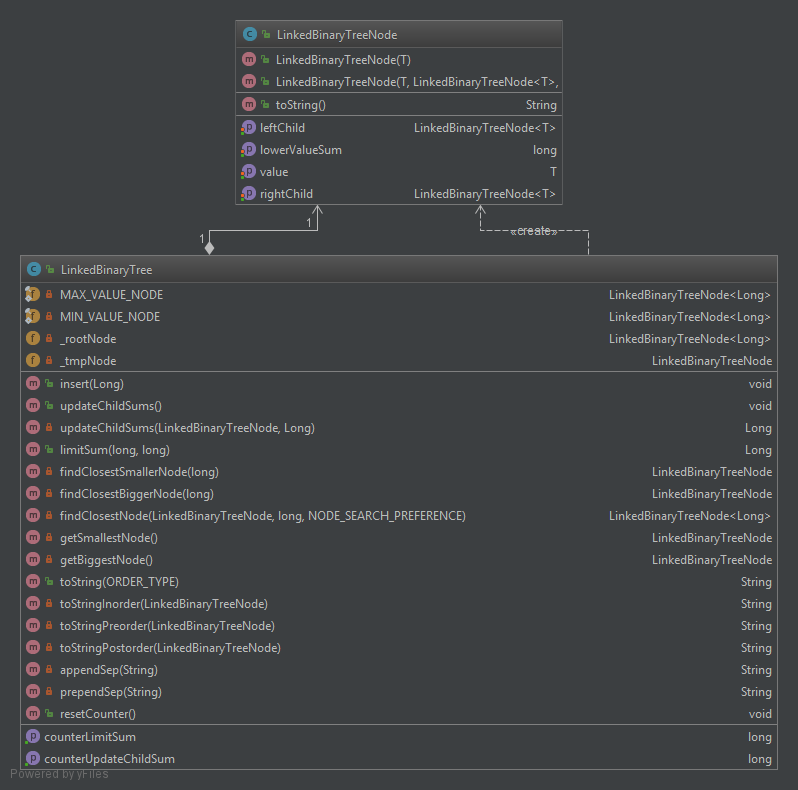
\includegraphics[scale=0.5]{classdiagram.png}
	\caption{UML-Klassendiagramm}
\end{figure}

\newpage
\section{Komplexitätsuntersuchung}
Es wurde eine empirische Komplexitätsuntersuchung durchgeführt, bei welcher binäre Suchbäume aus $N$ Elementen mit $N = 10^k$ mit $k = 1,\ldots,6$ erzeugt wurden. Für jede Größe $N$ wurden 100 Durchläufe durchgeführt. Es wurden die benötigten Instruktionen der Methoden \javainline{updateChildSums()} sowie \javainline{limitSum()} aufgezeichnet.\\
\\
Hierbei ergaben sich folgende Ergebnisse:

\subsection{Ergebnisse \javainline{updateChildSums()}}

Es zeigt sich, dass die benötigten Instruktionen für die Berechnung der Anzahl der im Baum vorhandenen Elemente entspricht. Die Diskrepanz zur Anzahl der Eingangselemente $N$ ergibt sich dadurch, dass durch die zufällige Generierung der Zahlen auch doppelte Elemente vorkommen, welche aber nur jeweils einmal in den Baum eingefügt werden. Somit ergibt sich für \javainline{updateChildSums()} eine Komplexität von $\mathcal{O}(N)$.

\begin{figure}[H]
	\centering
	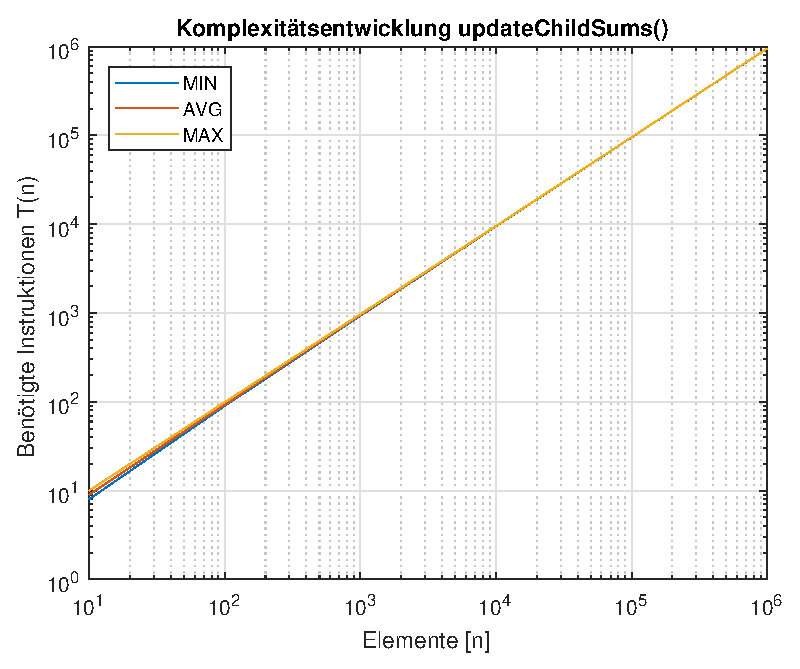
\includegraphics[scale=1]{komplexitaetsentwicklung_updateChildSums.eps}
	\caption{Instruktionen \javainline{updateChildSums()}}
\end{figure}

\begin{table}[H]
	\centering
	\begin{tabular}{ l | r | r | r }
		\textbf{N} & \textbf{MIN} & \textbf{AVG} & \textbf{MAX}\\
		\hline\hline
		$10^1$	&	8 & 9 & 10	\\ \hline
		$10^2$	& 90 & 93	& 99	\\ \hline
		$10^3$	& 930 & 945 & 969	\\ \hline
		$10^4$	& 9469 & 9514 & 9555	\\ \hline
		$10^5$	& 95001 & 95135 & 95284	\\ \hline
		$10^6$	& 951149 & 951694	& 952130 \\ \hline
	\end{tabular}
	\caption{Instruktionen \javainline{updateChildSums()}}
\end{table}

\subsection{Ergebnisse \javainline{limitSum()}}
Zum Bestimmen der Summe müssen lediglich die zwei Knoten gefunden werden, welche das Intervall einschließen. Somit wird die Komplexität auf das Suchen von Knoten in einem binären Suchbaum reduziert. Hiermit ergibt sich für \javainline{limitSum()} eine Komplexität von $\mathcal{O}(log(n))$.

\begin{figure}[H]
	\centering
	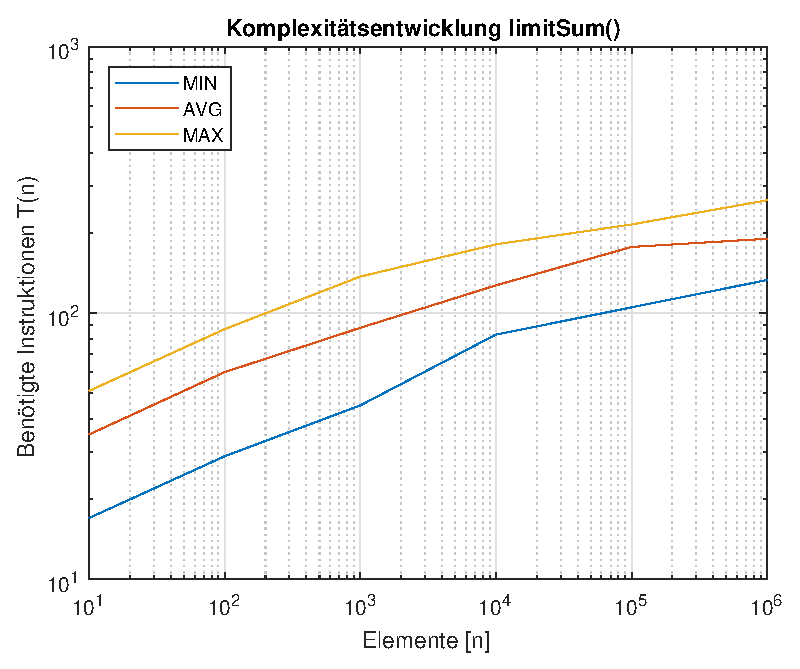
\includegraphics[scale=1]{komplexitaetsentwicklung_limitSum.eps}
	\caption{Instruktionen \javainline{limitSum()}}
\end{figure}

\begin{table}[H]
	\centering
	\begin{tabular}{ l | r | r | r }
		\textbf{N} & \textbf{MIN} & \textbf{AVG} & \textbf{MAX}\\
		\hline\hline
		$10^1$	&	17 & 35 & 51	\\ \hline
		$10^2$	& 29 & 60	& 87	\\ \hline
		$10^3$	& 45 & 88 & 137	\\ \hline
		$10^4$	& 83 & 127 & 181 \\ \hline
		$10^5$	& 105 & 177 & 215	\\ \hline
		$10^6$	& 133 & 190	& 265 \\ \hline
	\end{tabular}
	\caption{Instruktionen \javainline{limitSum()}}
\end{table}

\subsection{Anmerkungen}
Die zu analysierenden binären Suchbäume wurden wie folgt erzeugt:

\begin{javacode}
private static LinkedBinaryTree generateTree(long size) {
	LinkedBinaryTree tree = new LinkedBinaryTree();
	
	// Fill random values
	for (long i = 0; i < size; i++) {
		tree.insert((long) (Math.random()*size*10));
	}
	
	return tree;
}
\end{javacode}


\end{document}